The minimap was implemented to give the player a better overview of the map and its entities.
For the ``minimap'', two different implementation are explored. 
The initial implementation was developed during prototyping sessions to show the feasibility and usefulness of having a minimap in-game. 
This initial implementation was however encumbered by sub-par performance.
The optimized implementation transferred part of the calculations to the GPU, thereby gaining better performance.

\subsection{Initial implementation}
The minimap implementation was initially inspired by \textit{bitmap-blitting}
techniques used in \textit{older} games\cite{bitmap-blitting}, which means that the general idea for
the implementation is to \textit{blit} - or plot - individual pixels to a
texture, corresponding to specific types of tiles or entities. This means that
there are several variable factors that needs to be considered:
\begin{itemize}
    \item The current position of the player
    \item The position of enemies within the game 
    \item What pixel-color to use when plotting the background and entities
\end{itemize}
Having all enemies and players managed in singleton-accessible instances,
makes it easy to satisfy the two first items on the list. The last item
however, we want to be able to define in a flexible way. This
has to do with the fact that any map can be loaded with any given
texture pack, meaning that walls, ground, grass and so on, appear differently
in the game, depending on the texture pack used.
We solved the problem by following the colors defined on the map in the texture pack as shown in figure \ref{minimap:colordefinition}.
\\
\begin{figure}
	\centering
    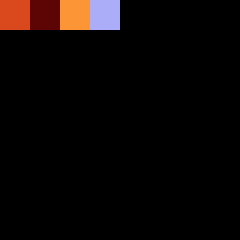
\includegraphics[scale=.5]{figures/minimap/minimap_colors.png}
    \caption{The image defining the colors to be used in the minimap.}
    \label{minimap:colordefinition}
\end{figure}

The colors used for plotting entities and the background on the minimap are
defined in a \texttt{PNG} image, accompanying the selected texture pack for that
map. The colors are parsed by index, e.g. the first pixel defines ground
color, second pixel defines grass color and etc.
\\
\\
The entities and background is blitted onto a texture at a shifted position, in
order to represent the players current position on the map. If entities such as
enemies and other players are within the players view bounds of the
texture, they are blitted onto the minimap textures as well as shown in figure \ref{minimap:enemies}.
\\
\begin{figure}
	\centering
    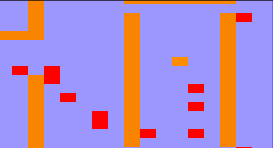
\includegraphics[scale=.5]{figures/minimap/enemies_on_minimap.png}
    \caption{Enemies shown as red squares on the minimap.}
    \label{minimap:enemies}
\end{figure}

As mentioned in the beginning of this chapter, the implementation just
described proved to have performance implications, which was partly expected. 
This has to do with the performance overhead of blitting the whole texture every time something changed.
Whether that was due to the camera position or an entity that changed position.
This had a big cost of CPU time because the CPU had to recalculate each pixel on the map all the time.


\subsection{Optimized implementation}
In order to optimize our minimap it was important to avoid the recalculation of texture each time something changed.
To do so a new approach was applied.

The new approach is based on offsetting the texture instead of recalculate a new texture all the time.
By doing so we believe that the offset calculation of the texture is transferred to the GPU instead of happening on the CPU.
This is done by adding a \textit{RawImage} to a \textit{game object} with a canvas renderer.
The \textit{RawImage} contains the properties:
\begin{itemize}
\item Texture
\item Color
\item Material
\item UV Rectangle
\end{itemize}
The texture will be our full map, and the UV Rectangle will be used to offset and control the size of the minimap, as shown in Figure \ref{minimap:creation}.
\begin{figure}[H]
    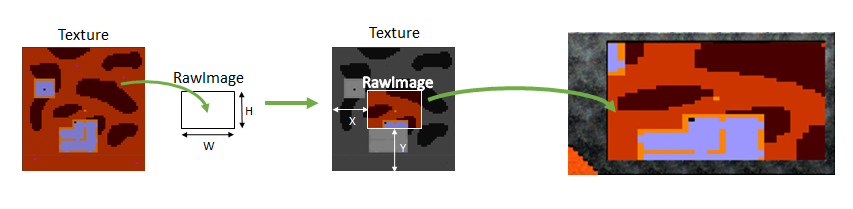
\includegraphics[width = \textwidth]{figures/minimap/RawImage.png}
    \caption{Illustration of the minimap creation and control}
    \label{minimap:creation}
\end{figure}

The task which the CPU is still required to do is:
\begin{itemize}
\item Give the \textit{RawImage} a size and width relative to the map
\item Calculate the offset that is required for the player to be inside the minimap
\item Plotting entities on the texture
\end{itemize}
Modifying the size of the \textit{RawImage} is relatively easy. 
To do so you have the UV Rectangle which contains a height and a width property:
\begin{itemize}
\item The Height (H) - Height of the what should be shown, represented in a ratio of the full height of the texture given from 0 to 1
\item The Width (W) - Height of the what should be shown, represented in a ratio of the full height of the texture given from 0 to 1
\end{itemize}
From here one can convert the height and width of the map into a vector and normalize it which gives a  ratio aspect of the height and width. Which then can be scaled to represent the desired \textit{RawImage}.

The UV Rectangle is also used to control the offset from the button left corner, this is done by changing the values:
\begin{itemize}
\item X - Which controls the offset on the x-axis
\item Y - Which controls the offset on the y-axis
\end{itemize}
In order to determine the offset that makes the player stay inside the RawImage, two simple equations are used\\
$\textit{Offset}_x = \frac{playerPosition.x}{Minimap.width} \cdot \textit{maxOffset}$\\
$\textit{Offset}_y = \frac{playerPosition.y}{Minimap.width} \cdot \textit{maxOffset}$\\
The last task was to add the different entities to the texture. 
In order to do so an a copy of the untouched map is created and a dictionary which uses an entity as key and a position as value.
When a entity is plotted onto the minimap the entities' position is store in the dictionary.
The next time the minimap then updates it checks whether a entity has moved or died, if so the old position is recolored back to its original color using the untouched map, and the new position is color with the color of the entity.
